\documentclass[letterpaper,12pt]{article}
\usepackage{listings} %For code in appendix
\usepackage{color}
\usepackage{appendix}
\usepackage{tabularx} % extra features for tabular environment
\usepackage{amsmath}  % improve math presentation
\usepackage{graphicx} % takes care of graphic including machinery
\usepackage[margin=1in,letterpaper]{geometry} % decreases margins
\usepackage{cite} % takes care of citations
\usepackage[final]{hyperref} % adds hyper links inside the generated pdf file
\usepackage{float}
%\usepackage{pythonhighlight}

\hypersetup{
	colorlinks=true,       % false: boxed links; true: colored links
	linkcolor=blue,        % color of internal links
	citecolor=blue,        % color of links to bibliography
	filecolor=magenta,     % color of file links
	urlcolor=blue         
}
\usepackage{blindtext}

\lstset
{ %Formatting for code in appendix
    language=Python,
    basicstyle=\footnotesize,
    numbers=left,
    stepnumber=1,
    showstringspaces=false,
    tabsize=1,
    breaklines=true,
    breakatwhitespace=false,
}
%++++++++++++++++++++++++++++++++++++++++


\begin{document}
\title{DAT510-1 20H Network security and vulnerability. Assignment 3. Digital Signature implementation}
\author{Asahi Cantu Moreno (student id: 253964)}
\date{\today}
\maketitle

\begin{abstract}
With the implementation of encryption algorithms and key exchange mechanisms, it is important now to make use of the digital signature standards for message authentication  and verification and implement the non-repudiation principle as well. This report explains the implementation of such digital signature schemes and its implementation via python code for a chat messages application able to share public keys and verify a message or a file once it has been received. A PKI\footnote{Public Key Infrastructure, A set of policies, processes, server platforms, software and workstations used for the purpose of administering certificates and public-private key pairs, including the ability to issue, maintain, and revoke public key
certificates\cite{WS2017-PKI}} is implemented, where it is assumed that there is already a trusted authority in charge of verifying that the public key shared from user to user is authentic and information exchange is reliable. Creation of public and private keys per user is created in an asymmetric way, where both users create their own public and private keys and then they share such public keys and a signature of the given information, where it is lately hashed and verified against the original message encrypted with the public key. The RSA\footnote{The RSA scheme is a cipher in which the plaintext and ciphertext are integers
between 0 and n - 1 for some n. A typical size for n is 1024 bits, or 309 decimal
digits. That is, n is less than 21024. We examine RSA in this section in some detail,
beginning with an explanation of the algorithm. Then we examine some of the computational and cryptanalytical implications of RSA. \cite{WS2017-RSA}} algorithm of 1024 bits was implemented.  
The whole schema consists of:
\begin{enumerate}
    \item A Trusted Authority server. Validates and certifies that public keys shared among users are trusted and valid
    \item An end point terminal messenger application per user. Each user connects to the trusted server and then the application creates the corresponding RSA keys, where later the public key is shared once the handshake for two users is performed to begin a chat session. With these shared keys it is possible now to send information and verify its authenticity.
    
\end{enumerate}

The results applied for this application demonstrate that messages can be easily transmitted over the network and be validated as long as the public key is known and it is confirmed that such public key belongs to the entity in questions. This is now a standard for secure web communications, and in conjunction with different symmetric encryption algorithms and other key exchange protocols is possible to create secure channels where only two entities know the deciphered information.
\end{abstract}
\newpage
\section{Introduction}
    \subsection{Background}
    To understand and implement these processes it was necessary to have knowledge on the different symmetric encryption algorithms as well as key-exchange mechanisms and asymmetric implementations used in the modern world. The strength of such algorithms relies on the infeasibility to perform brute force attacks to find the private key or plaint text due to the length of such key and complexity of the algorithms.
    \subsubsection{Symmetric encryption}
    It is nowadays very common to use this mechanism with where a block of information is processed with an algorithm and a secret key. Also referred to as conventional encryption or single-key
encryption, was the only type of encryption in use prior to the development of public key encryption in the 1970s. It remains by far the most widely used of the two types
of encryption.\footnote{AES, DES, RC6, Blowfish are amongst the strongest algorithms.}\cite{WS2017-SYMENC}
    \subsubsection{Asymmetric encryption}
    The mathematical discovery and subsequent implementation of public and private keys represented a major breakthrough in the history of information security and cryptography. Public-key cryptography provides a radical departure from all that has gone before. For one thing, public-key algorithms are based on mathematical functions rather than on substitution and permutation. More important, public-key cryptography is asymmetric, involving the use of two separate keys, in contrast to symmetric encryption, which uses only one key. The use of two keys has profound consequences in the areas of confidentiality, key distribution, and authentication. \cite{WS2017-PKI}. Asymmetric algorithms rely on one key for encryption and a different but related key for decryption.
    \begin{figure}[H]
    \centering
    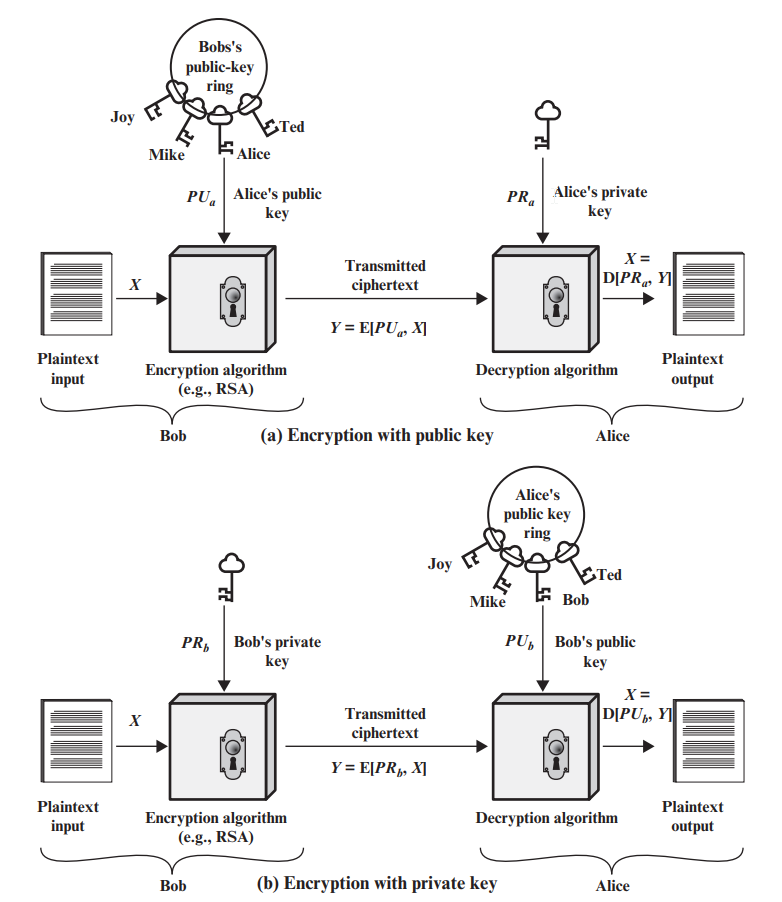
\includegraphics[width=0.9\textwidth]{assets/asymk.png}
    \caption{Public and private key encryption schemes.}
    \label{fig:CRP_CHAT}
\end{figure}
    \subsubsection{RSA Algorithm}
    The RSA scheme\footnote{Rivest-Shamir-Adleman scheme asymmetric algorithm\cite{WS2017-RSA}} is a cipher in which the plaintext and ciphertext are integers between 0 and n-1 for some n. A typical size for n is 1024 bits, or 309 decimal digits. That is, n is less than 21024. RSA makes use of an expression with exponentials. Plaintext is encrypted in blocks,
with each block having a binary value less than some number n. The RSA algorithm creates and publishes a public key based on two large prime numbers, along with an auxiliary value. The prime numbers are kept secret. Messages can be encrypted by anyone, via the public key, but can only be decoded by someone who knows the prime numbers. The security of RSA relies on the practical difficulty of factoring the product of two large prime numbers, the "factoring problem". Breaking RSA encryption is known as the RSA problem.
    \subsubsection{SHA-512}
Known also as SHA-2\footnote{Secure Hash Algorithm} and developed by the National Institute of Standards and Technology (NIST) and published as a federal information processing standard (FIPS 180) in 1993. It is a replacement of SHA (now known as SHA-0) and SHA-1. The actual standards document is entitled
“Secure Hash Standard". SHA-512 uses the same types of modular arithmetic and logical binary operations as SHA-1 and it is widely used for multiple application protocols such as TLS, SSL, PGP, SSH. The algorithm generates a 512-bit (32-bytes) signature given an information block, which is collision strong and reliable for message reliability and authenticity verification when sending it over the network.
 \subsubsection{PKI}
    PKI\footnote{Public Key Infrastructure} is defined as the set of hardware, software, people, policies, and procedures needed to create, manage, store, distribute, and revoke digital certificates based on asymmetric cryptography. The principal objective for developing a PKI is to enable secure, convenient, and efficient acquisition of public keys. 
 \begin{itemize}
     \item End entity: refers to any final user, device or element that can be identified in the subject field of a public-key certificate.
     \item Certification authority (CA): The issuer of certificates and (usually) certificate revocation lists (CRLs).
     \item Registration authority (RA): An optional component that can assume some functions from the CA. Often associated with the end entity registration process and other areas.
    \item CRL\footnote{A Certificate Revocation List (CRL) is a list of digital certificates that have been revoked by the issuing Certificate Authority (CA) before their scheduled expiration date and should no longer be trusted. CRLs are a type of blacklist and are used by various endpoints, including Web browsers, to verify whether a certificate is valid and trustworthy. Digital certificates are used in the encryption process to secure communications, most often by using the TLS/SSL protocol. The certificate, which is signed by the issuing Certificate Authority, also provides proof of the identity of the certificate owner.\cite{CRL}} issuer: An optional component that a CA can delegate to publish CRLs.
    \item Repository: A generic term used to denote any method for storing certificates and CRLs so that they can be retrieved by end entities.
 \end{itemize}

With all those theorietical definitions and algorithms it the implementation of the digital signature scheme using RSA for public  and private key generation, SHA-512 as a digital signature and PKI as a simple server and end entities to share and keep the public keys were implemented.
        
    

\section{Design and implementation}
The following implementation in figure \ref{fig:dss_scheme} was implemented for the final application.
\begin{figure}[H]
    \centering
    \includegraphics[width=0.9\textwidth]{assets/dss.png}
    \caption{Digital signature scheme implementation.}
    \label{fig:dss_scheme}
\end{figure}
\subsection{Schema implementation}
    \subsubsection{Server.}
    Because a simple PKI infrastructure was implemented for the digital signature and verification mechanisms, a simple server holding the public keys and verifying public key ownership per user was implemented. Such server was developed in python code and using flask/flask.socketio as communication protocols for the end entities in the message exchange. The server works as an end-to-end communication entity assuming both users messaging each other are entering over a secure channel trusting the server to share their public keys.

    \subsubsection{End entity.}
    Consists of a GUI\footnote{Graphical User Interface} which emulates a user connecting to the server over a secure channel where a Public and private keys are generated using RSA algorithm. Once the server authorizes the connection. Then, and once it has established communication with another user, their public keys are shared and now ready to send messages. The messages are signed using SHA-512 algorithm and all the information sent to the endpoint, where later can be verified by comparing the signature and the message ciphered with the public key. In addition to this, each user can send files over the network, regardless its size and because such file is divided into blocks once it is signed, it can be sent as well and later on verified by the final user. Files are also stored on each end point and all information is logged according to the final entity in place.


\subsection{Code implementation}
Different classess and files were created to perform and create the DSS mechanism:
\subsubsubsection{Python files created:}
\begin{enumerate}
    \item Server.py - Controls end-to-end entity connectivity and coordinates correct message exchange with corresponding public keys and signatures.
    \item Client.py - GUI that contains the mechanisms to connect to the server, generate asymmetric keys and sing the information wich later can be verified.
    \item DSS.py - Contains the implementation of RSA key generation and SHA-512 implementation for message signature. It is the cryptographic backbone of this implementation as it provides all the encryption mechanisms to make the application and server operate. By default RSA-1024 and SHA-512 have been chosen for message signature and verification.
    \item Log files, each entity (Server and clients) log all the information depending on the message exchange and encryption mechanisms.
\end{enumerate}
\subsubsubsection{DSS.py Code}
\hline
\begin{lstlisting}
#%%
'''
Author: Asahi Cantu Moreno
Descriptipn: DSS is a class for Digitas Signature Schema, implementing RSA Algorithm for message signature
'''
from Cryptodome.PublicKey import RSA
from Cryptodome.Cipher import PKCS1_OAEP
from Cryptodome.Signature import PKCS1_v1_5
from Cryptodome.Hash import SHA512, SHA384, SHA256, SHA, MD5
from Cryptodome import Random, PublicKey
from base64 import b64encode, b64decode

def newkeys(keysize):
   random_generator = Random.new().read
   key = RSA.generate(keysize, random_generator)
   private, public = key, key.publickey()
   return public, private

def extract_priv_key(priv_key):
    n = priv_key.n
    e = priv_key.e
    d = priv_key.d
    p = priv_key.p
    q = priv_key.q
    u = priv_key.u
    return (n, e, d, p, q, u)

def extract_pub_key(pub_key):
    n = pub_key.n
    e = pub_key.e
    return {'n':n,'e':e}

def create_pub_key(pub_key_dict):
    n = pub_key_dict['n']
    e = pub_key_dict['e']
    return RSA.RsaKey(n=n,e=e)

def rebuild_pub_key(components):
    n = components.n
    e = components.e
    d = components.d
    p = components.p
    q = components.q
    u = components.u
    return PublicKey.RsaKey(n=n, e=e, d=d, p=p, q=q, u=u)


def encrypt(message, pub_key):
   cipher = PKCS1_OAEP.new(pub_key)
   return cipher.encrypt(message)

def decrypt(ciphertext, priv_key):
   cipher = PKCS1_OAEP.new(priv_key)
   return cipher.decrypt(ciphertext)

# Authorization
def sign(message, priv_key):
    signer = PKCS1_v1_5.new(priv_key)
    digest = SHA512.new()
    digest.update(message)
    return signer.sign(digest)

#Authentication
def verify(message, signature, pub_key):
    signer = PKCS1_v1_5.new(pub_key)
    digest = SHA512.new()
    digest.update(message)
    verified = signer.verify(digest, signature)
    return verified
\end{lstlisting}
\hline


\subsection{Part II. Implementation of Secure Chat messenger.}
By confirming the developed algorithm works it was now required to implement a simple chat application that operates with the key exchange and encryption mechanisms previously developed.
For this implementation the same methodology as in Part I applies, with the creation of a server and client applications.

In figure \ref{fig:CRP_CHAT} a simulation of the program shows the results of the messaging exchange system.

\begin{figure}[H]
    \centering
    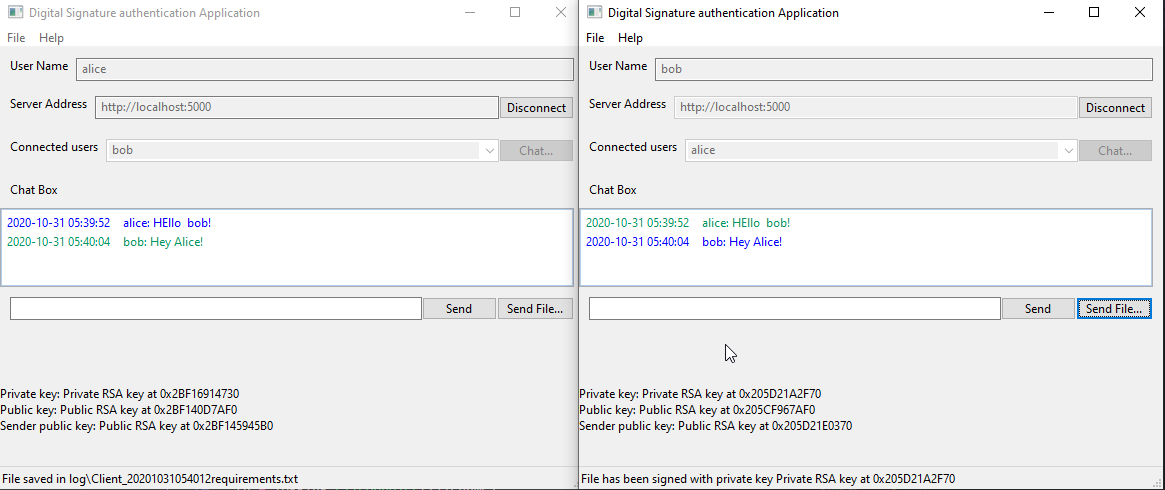
\includegraphics[width=0.9\textwidth]{assets/CryptoChat.png}
    \caption{Emulation of chat where each message or file sent is verified against a digital signature given a public key.}
    \label{fig:CRP_CHAT}
\end{figure}

\section{Test Results}
\subsubsection{Log files}
In the following images the log for each entity is presented.

\begin{figure}[H]
    \centering
    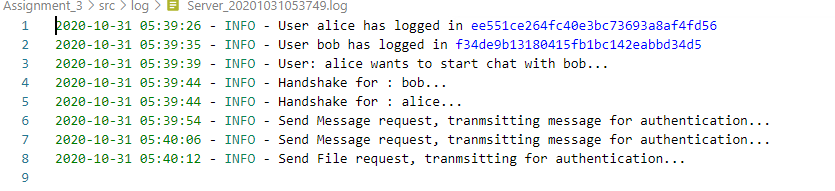
\includegraphics[width=0.9\textwidth]{assets/server_log.png}
    \caption{The log generated for the server entity.}
    \label{fig:SRV}
\end{figure}
\begin{figure}[H]
    \centering
    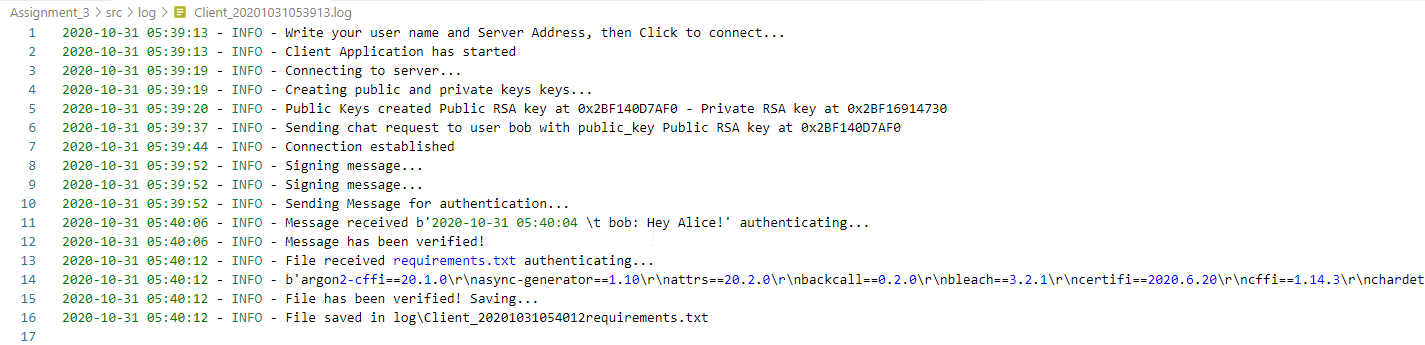
\includegraphics[width=0.9\textwidth]{assets/alice_log.png}
    \caption{The log generated for 'alice' client entity.}
    \label{fig:ALC}
\end{figure}
\begin{figure}[H]
    \centering
    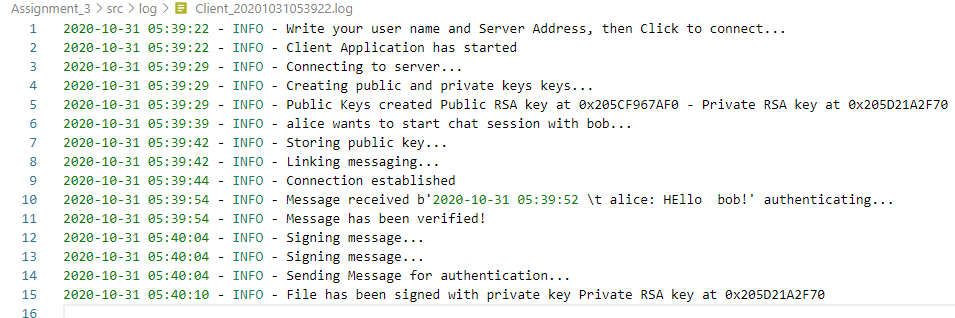
\includegraphics[width=0.9\textwidth]{assets/bob_log.png}
    \caption{The log generated for 'bob' client entity.}
    \label{fig:BOB}
\end{figure}


\section{Discussion}
A PKI infrastructure involves several entities where for its construction several features such as encryption algorithms, communication protocols, reliability and trust channels have to be predefined to make a secure and reliable connection. It is possible to see nowadays (and at the same time impressive to realize such changes have happened over the previous 20 years) a secure web browsing involves an https:, a trusted authority and every web site has a certificate which is basically the public key hosted by a trusted server and downloaded once the server gets the domain name over a DNS and point to the specific certificate. Once all this information has been established and acknowledged it is possible to start a secure browsing. In this case the implemented server acts as a trusted certificate authority where each final entity connects and share their own public key. It is through this mechanism that messages can be singed to later be verified and acknowledge the precedence of the information. The concept of digital signature is vital for the development of the world and the virtualization of systems where non repudiation is vital and important for the industry and its processes.


\section{Part II}
PKI certificates are documents that act as digital passports, assigned to any entity that wants to participate
in a PKI-secured conversation. They can include quite a bit of data. the main part of it normally consists
of a public key. There are several PKI implementations however the most popular public key
infrastructure system is TLS/SSL protocol, which secures just about all encrypted HTTP communication
in the whole internet \cite{TLS_Internet_Society}.

\subsection{What are the different types of SSL's and how different they are in aspect of security? Why ?}
SSL stands for Secure Sockets Layer, it was released under three different versions and although is no longer used by any institution because of its proven security flaws, the new implementation TLS (Transport  Layer Security) sits on its basic principles and implements several improvements for SSL. It is nowadays know as SSL/TLS. It consists of a several other protocols and encryption algorithms for key exchange, signature, verification and authentication. 

\begin{figure}[H]
    \centering
    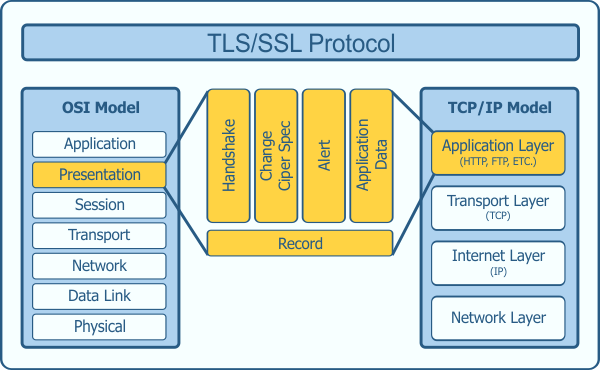
\includegraphics[width=0.9\textwidth]{assets/TLS-added.png}
    \caption{TLS PRotocol.\cite{IOT_SSL}}
    \label{fig:TLS}
\end{figure}

Among its different functions, TLS does the following:

\begin{itemize}
\item Separating key agreement and authentication algorithms from the cipher suites
\item Removing support for weak and less-used named elliptic curves
\item Removing support for MD5 and SHA-224 cryptographic hash functions
\item Requiring digital signatures even when a previous configuration is used
\item Integrating HKDF and the semi-ephemeral DH proposal
\item Replacing resumption with PSK and tickets
\item Supporting 1-RTT handshakes and initial support for 0-RTT
\item Mandating perfect forward secrecy, by means of using ephemeral keys during the (EC)DH key agreement
\item Dropping support for many insecure or obsolete features including compression, renegotiation, non-AEAD ciphers, non-PFS key exchange (among which are static RSA and static DH key exchanges), custom DHE groups, EC point format negotiation, Change Cipher Spec protocol, Hello message UNIX time, and the length field AD input to AEAD ciphers
\item Prohibiting SSL or RC4 negotiation for backwards compatibility
\item Integrating use of session hash
\item Deprecating use of the record layer version number and freezing the number for improved backwards compatibility
\item Moving some security-related algorithm details from an appendix to the specification and relegating ClientKeyShare to an appendix
\item Adding the ChaCha20 stream cipher with the Poly1305 message authentication code
\item Adding the Ed25519 and Ed448 digital signature algorithms
\item Adding the x25519 and x448 key exchange protocols
\item Adds support for sending multiple OCSP responses
\item Encrypts all handshake messages after the ServerHello
\end{itemize}

SSL/TLS uses strong algorithms for encryption and key exchange and is used by other different communications protovols such as:
\begin{itemize}
    \item HTTPS (HTTP Over SSL/TLS)
    \item VOIP (Voice Over IP)
\end{itemize}

This way TLS is much stronger over SSL
\begin{figure}[H]
    \centering
    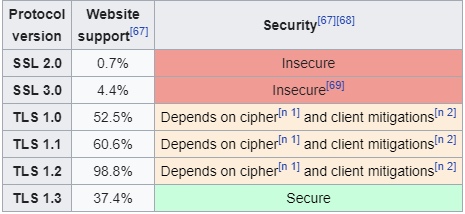
\includegraphics[width=0.9\textwidth]{assets/tlsssl.png}
    \caption{SSL/TLS security and state of the art.\cite{WIKI_TLS}}
    \label{fig:SSLTLS}
\end{figure}

\subsection{Research about the the Certificate Authority Security concerns and explain.}
A Certificate authority (CA) is a global entity trust by many enterprises whose main role is to emit digital certificates (Public keys corresponding to specific companies, defining their ownership, expiration date and applicable domains). Such certificates are defined by the X.509 standard and are commonly used for the HTTPS protocol. The weakness of the CA and the reason while it has failed several times after its implementation (specially in year 2011) relies on the vulnerabilities of the CA's Systems, security protocols and human factors. If for some reason a hacker manages to break into the CA's IT Systems or some of their personnel through some sort of social engineering ro bribe it is certain enough to say that the authority is very vulnerable and at big risk due to the fact that the third partie's private keys could be discovered or new certificates could be spoofed. In this case and since TLS reles under CA for certificate issuance and trustworthy, is therefore the weakest link in the TLS chain \cite{CA_INFOSEC}.
\subsection{How does browsers identify secure CA's From another CA's and how is it measured ?}
Browsers and modern operating systems come with a predefined CA's certificates list provided by th e major companies in charge of issuing such certificates. This way when a web browser tries to identify if a web site's certificate is signed by one of those major companies and then certify that the website can be trusted. If such certificate has an unknown authority or is self signed, the browser will show a warning message and might even prevent the user from browsing that web page unless the certificate authority is explicitly added to the trusted root certificate publishers.

Here is a detailed list of the steps a browser will follow to measure a certificate and rely on it\cite{SSL_CERT}:
\begin{enumerate}
    \item  The browser verifies the certificate’s integrity
The signature on the certificate can be verified using normal public key cryptography. If the signature is invalid, then the certificate is considered to be modified after its issuance and is therefore rejected.
\item The browser verifies the certificate’s validity
A certificate’s validity period is the time interval during which the signing CA warrants that it will maintain information about its status. Browsers reject any certificates with a validity period ending before or starting after the date and time of the validation check.
\item The browser checks the certificate’s revocation status
When a certificate is issued, it is expected to be in use for its entire validity period. Of course, various circumstances may cause a certificate to become invalid before it naturally expires. Use of Certificate Revocation Lists (CRL)

\item he browser verifies the issuer
Certificates are normally associated with two entities:

The issuer, which is the entity owning the signing key and
The subject, which refers to the owner of the public key that the certificate authenticates.
Browsers check that a certificate’s issuer field is the same as the subject field of the previous certificate in the path. For added security, most PKI implementations also verify that the issuer’s key is the same as the key that signed the current certificate. (Note that this is not true for the trust anchor, since roots are self-issued – i.e. they have the same issuer and subject.)

\item The browser checks name constraints
A privately owned (but publicly trusted) intermediate CA with the appropriate name constraints can provide an organization with fine-grained control over certificate management and issuance. Certificates can be limited to a specific domain or domain tree (i.e. including subdomains) for a company or organization’s domain name. Name constraints are often used for intermediate CA certificates purchased from a publicly trusted CA to prevent the intermediate CA from issuing perfectly valid certificates for third-party domains.

\item The browser checks policy constraints
A certificate policy is a legal document published by a CA, officially detailing the procedures they follow to issue and manage their certificates. CA's might issue a certificate under one or more policies, and links to these are included in each certificate issued so that relying parties can evaluate these policies before deciding to trust that certificate.

\item The browser checks basic constraints (a.k.a. path length)
The X.509 v3 format allows issuers to define the maximum path length a certificate can support. This provides control over how far each certificate can be placed in a certification path.

\item The browser verifies key usage
The “key usage” extension states the purpose of the key contained in the certificate. Browsers reject certificates violating their key usage constraints, such as encountering a server certificate with a key meant only for CRL signing.

\item The browser continues to process all remaining critical extensions
Browsers finally proceed to validate all remaining extensions that the current certificate designates as critical, before moving on to the next. If a browser reaches a path’s leaf certificate without error, then the path is accepted as valid. If any errors are produced the path is marked as invalid and a secure connection is not established.

\end{enumerate}




 
\section{Conclusion}
The implementation of such mechanisms in a simple manner show nothing but the complex world of cryptography and secure communication, the different parties, enterprises and entities that play a role in the security, and yet it is common to see there are so many times systems being hacked. It was possible to emulate and build a simple encyption comunication application to sign messages and allow its authentication by implementing python packages for RSA and SHA-512. Later on and through the use of Python language as well as socketio communication protocol it was possible to learn and confirm the importance of digital signatures for reliable and accurate communication as well as the considerable latency that strong encryption systems can generate. 
These tests were made on a normal computer without end-to-end communication, however the latency is perceptible for each communication mechanism. 

A very important lesson learned from this analysis is the realization that encryption algorithms are complex and they add an extra layer of complexity for building applications. That said, it is very important to have a quality control rule for communication processes and to think how far it is possible to get into these encryption systems without affecting the latency of the communication applications.

A video presentation has been elaborated and can be visualized \href{https://youtu.be/cKevoex-4h8}{in this link.}

\bibliographystyle{plainnat}
\bibliography{references}

\end{document}
